\documentclass{beamer}
\usetheme{Madrid}
\usepackage{lmodern}% http://ctan.org/pkg/lm
\setbeamersize{text margin left = 2.5em}
\setbeamersize{text margin right = 2.5em}
\usepackage{color}
\usepackage{graphicx}
\usepackage{MnSymbol}
\usepackage{amsmath}
\usepackage{comment}
\usepackage{tikz}
\usepackage{subfigure}
\usepackage{listings}
\usetikzlibrary{automata}

%\usepackage[backend=bibtex,sorting=none]{biblatex}
%\addbibresource{E:/Papers/LiuLab} %BibTeX�����ļ���λ��
%\setbeamerfont{footnote}{size=\tiny}
\setbeamertemplate{theorems}[numbered]
\setbeamertemplate{caption}[numbered]
%% ʹ�ý�ע���õ�Ƭijҳ���Ӳο����ס�
%% ��������ʹ�ã�\footfullcite{bib_item} %����item
%% \usepackage{anyfontsize}%% allowing font sizes at arbitrary sizes
\logo{
\includegraphics[height=0.05\textwidth]{Pic/logo}}
\newtheorem{df}{Definition}
\newtheorem{DF}{DEFINITION}
\newtheorem{prop}{Proposition}
\newtheorem{thm}{Theorem}
\newtheorem{cor}{COROLLARY}
\newtheorem{lm}{LEMMA}
% ----------------------------------------------------------------------------------------
% TITLE PAGE
% ----------------------------------------------------------------------------------------

\title{E10 Decision Tree and Naive Bayes}
% The short title appears at the bottom of every slide, the full title is only on the title page

\author{Suixin Ou} % Your name
\institute[SYSU] % Your institution as it will appear on the bottom of every slide, may be shorthand to save space
{
  School of Computer Science\\
  Sun Yat-sen University \\ % Your institution for the title page
  \medskip
  % Your email address
}

\date{December 14, 2021} % Date, can be changed to a custom date

\AtBeginSection[]
{
  \begin{frame}
    \tableofcontents[currentsection,currentsubsection]
  \end{frame}
}

\begin{document}

\begin{frame}
  \titlepage
\end{frame}

\begin{frame}
  \frametitle{Background}
  \begin{block}{The Adult Data Set}
    \begin{itemize}
    \item 
The UCI dataset (\url{http://archive.ics.uci.edu/ml/index.php}) is the most widely used dataset for machine learning. If you are interested in other datasets in other areas, you can refer to \url{https://www.zhihu.com/question/63383992/answer/222718972}.

    \item The Adult Data Set, sourced from the 1994 U.S. Census Income, is one of many UCI datasets. In this task, you should predict whether income exceeds \$50K per year based on census data.
    \end{itemize}
      
  \end{block}
\end{frame}



\begin{frame}
  \frametitle{Task}
  \begin{block}{Description}
	
    \begin{itemize}
      \item Dataset statistics

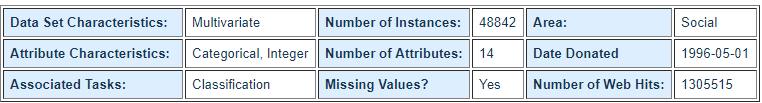
\includegraphics[width=0.85\textwidth]{Pic/dataset}
      \item Domain information

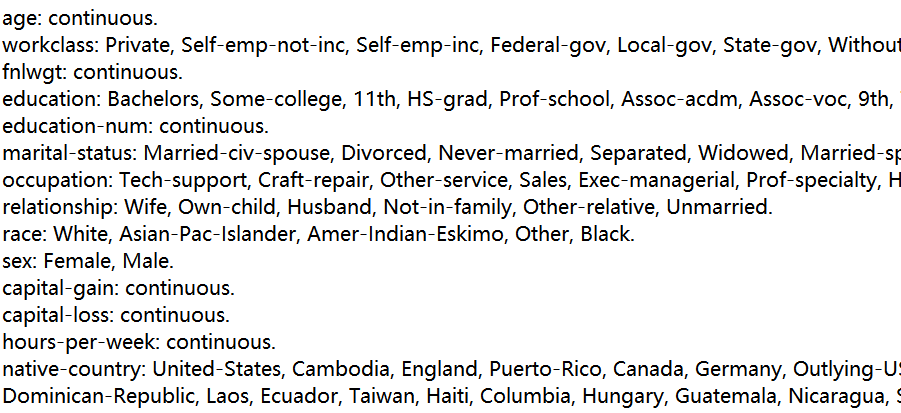
\includegraphics[width=0.85\textwidth]{Pic/domain}
% 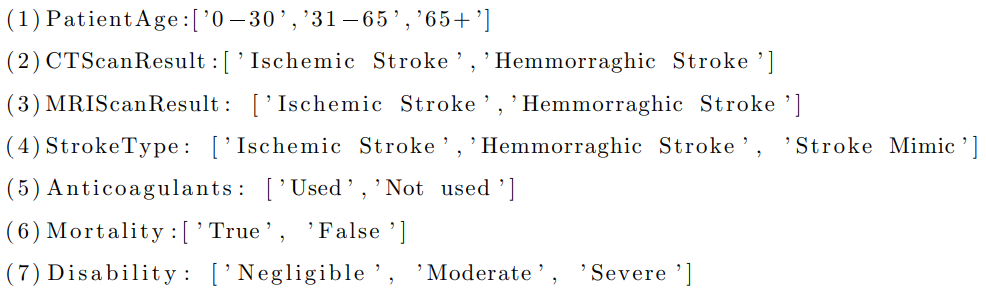
\includegraphics[width=10cm]{Pic/e21}
% 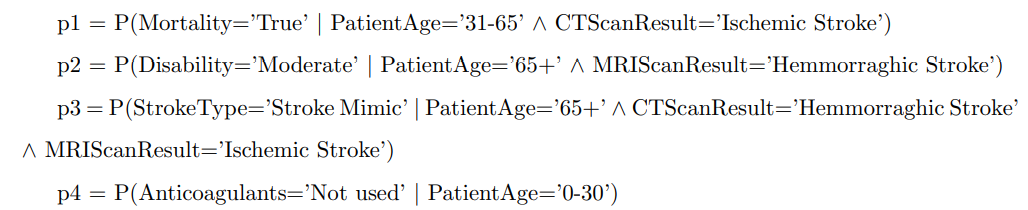
\includegraphics[width=10cm]{Pic/e22}
    \end{itemize}

  \end{block}
\end{frame}


\begin{frame}
  \frametitle{Solution}
      Read the file "adult.names"
      \\[10pt]
      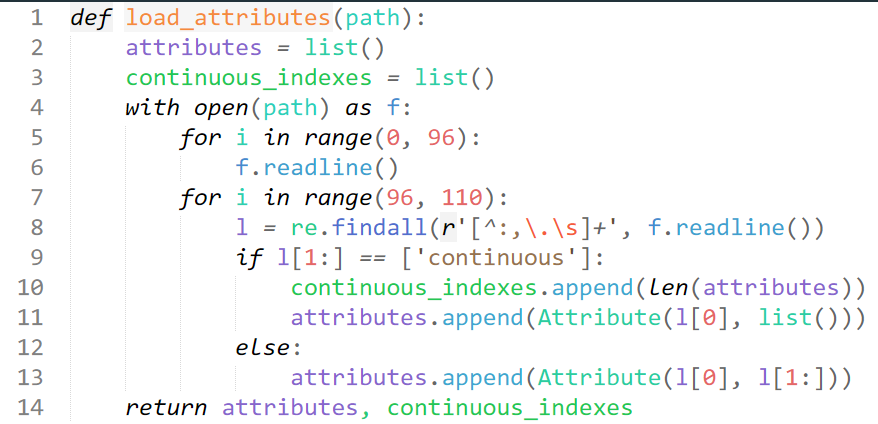
\includegraphics[width=1.0\textwidth]{Pic/input1}


\end{frame}

\begin{frame}
  \frametitle{Solution}

      Read the file "adult.data"
      \\[10pt]
      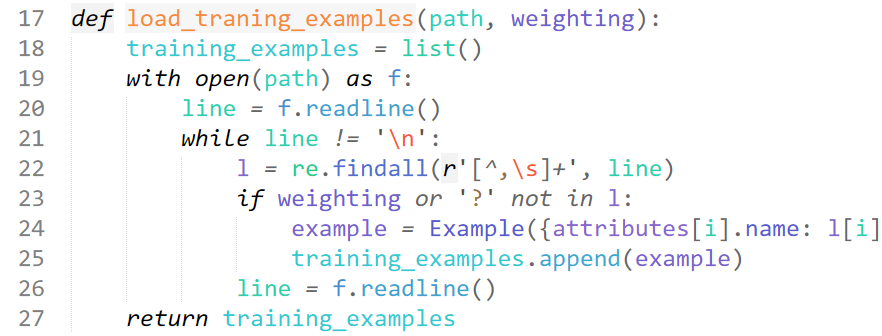
\includegraphics[width=1.0\textwidth]{Pic/input2}

\end{frame}

\begin{frame}
  \frametitle{Solution}
	  \textbf{Please Finish the DT/NB algorithm.}
      Read the file "adult.test" for testing
      \\[10pt]
      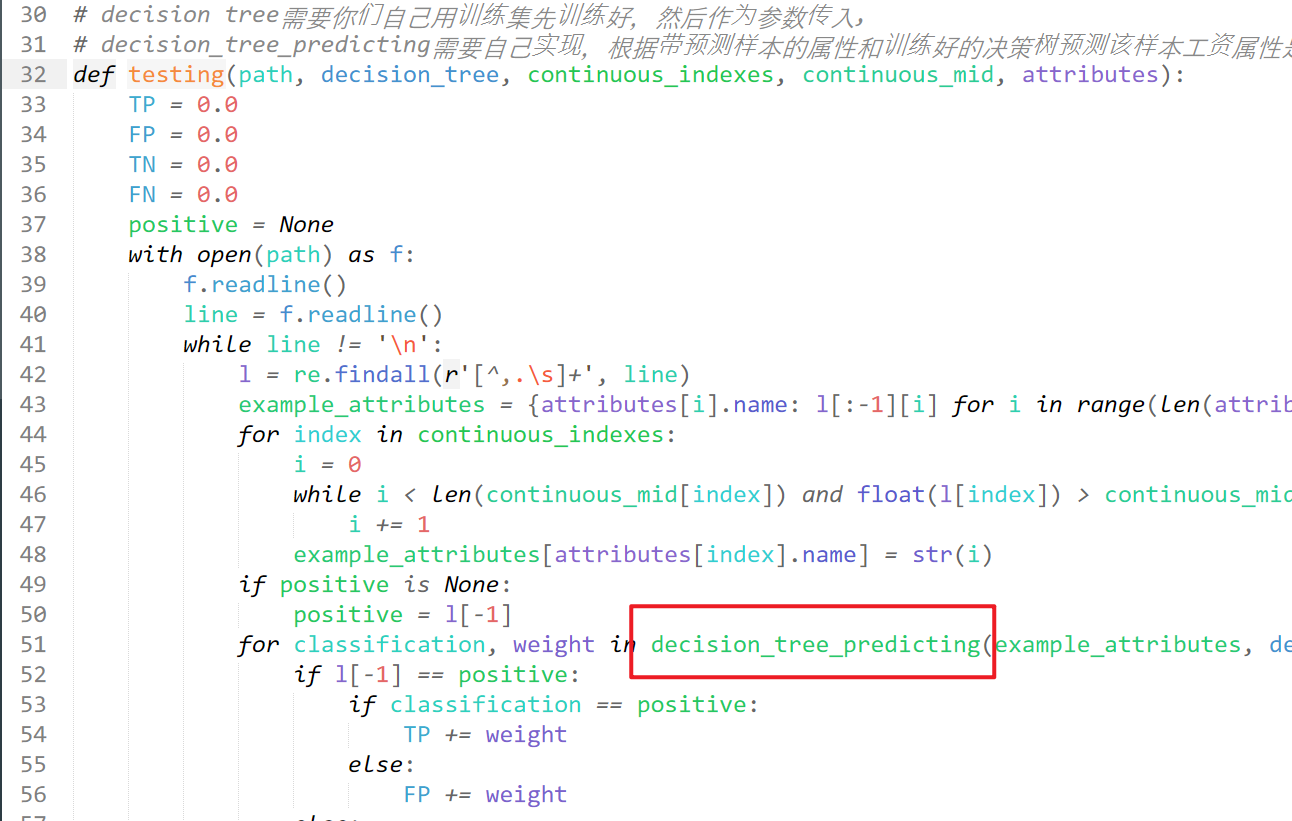
\includegraphics[width=0.9\textwidth]{Pic/output}

\end{frame}


\begin{frame}
  \frametitle{Submission}
  \begin{block}{Submission}
    pack your report \texttt{E10\_YourNumber.pdf} and source code into zip file \texttt{E10\_YourNumber.zip}, then send it to \texttt{ai\_course2021@163.com}.
  \end{block}
\end{frame}

%-----------------------------------------------------------------------------------------

\begin{frame}
  \Huge{\centerline{The End}}
\end{frame}

% ----------------------------------------------------------------------------------------


\end{document}
